\documentclass{beamer}

\mode<presentation>
{
  \usetheme{Warsaw}
  \setbeamercovered{transparent}
}
\usepackage[english]{babel}
\usepackage[utf8]{inputenc}
\usepackage{times}
\usepackage{float}
\usepackage[T1]{fontenc}

\title[PROYECTO - PYTHON] 
{M A Z E S}


\subtitle{}
\institute[ESCUELA SUPERIOR]
{	
	\centering
  		%
\includegraphics[totalheight=1in,width=1in]{ss}
  		
	ESCUELA SUPERIOR\\
	POLITECNICA DEL LITORAL
}
\date[CFP 2013]{Proyecto en Python, 2013}

\begin{document}
	\begin{frame}
  	  \titlepage
	\end{frame}
	
	%Integrantes del Grupo
	\begin {frame}{INTEGRANTES}
		 \begin{flushleft}
 			
\includegraphics[totalheight=1.2in,width=2in]{LTwitspol}
 		 \end{flushleft}
 		 
 		 \begin{itemize}
 		 	\item
				\begin{flushright} 		 		
 		 		Torres Criollo Daniel
 		 		\end{flushright}
 		 	\item
 		 		\begin{flushright}
 		 			Velez Gomez José
 		 		\end{flushright}
 		 \end{itemize}
  	\end{frame}
  	  	
  	%Seccion Introduccion
  	\begin{frame}{DESCRIPCION DEL JUEGO}
  		\centering
  		%
\includegraphics[totalheight=1in,width=1in]{ss}	
  		\begin{block}{}
  		Consiste en pasar tres niveles de laberintos con diferentes obstaculos, donde cada obstaculos estan representadas con moneditas que al tocarlas pueden hacerte regresar al inicio o culminar el juego. Ganas el fue cuando termine de pasar los tres niveles.
  		
  		\end{block}				
	\end{frame}

		
	\begin{frame}{DESARROLLO DEL JUEGO}
		\centering
  		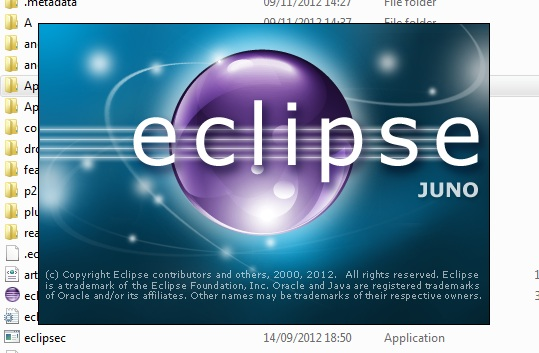
\includegraphics[totalheight=1.8in,width=2.5in]{ecliipse}	
  						
	\end{frame}

	\begin{frame}{EJECUTANDO LA APLICACION}
		\centering
  		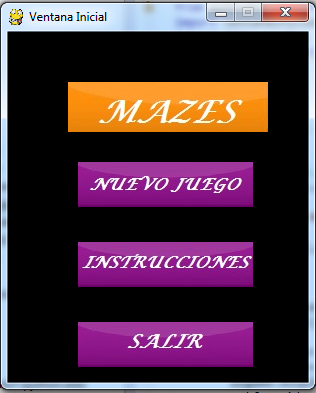
\includegraphics[totalheight=2.5in,width=1.5in]{Menu}	
  		
	\end{frame}

	\begin{frame}{EJECUTANDO LA APLICACION}
		\centering
  		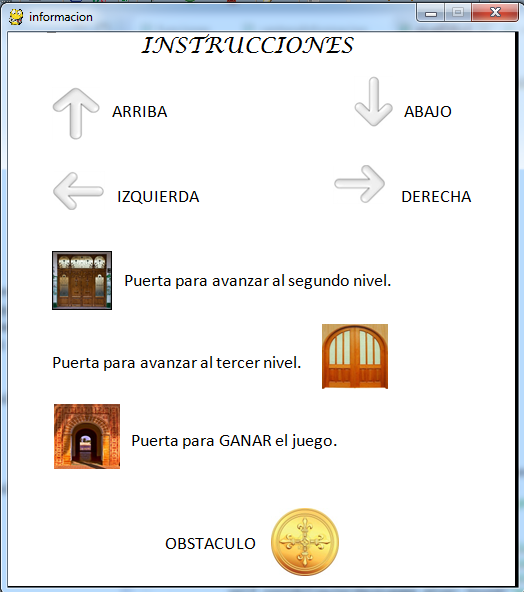
\includegraphics[totalheight=2.5in,width=1.5in]{Instrucciones}
  		
 	\end{frame}

\begin{frame}{EJECUTANDO LA APLICACION}
		\centering
  		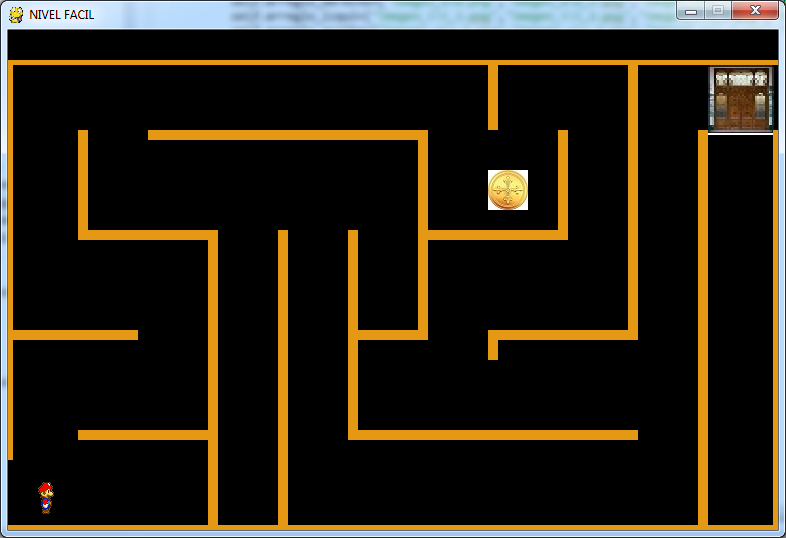
\includegraphics[totalheight=2.5in,width=2.5in]{juego}	
  		
 	\end{frame}

		
	%\appendix	
	%\section<presentation>*{\appendixname}
	\subsection<presentation>*{MAZES -- PYTHON}
	\begin{frame}
	\centering
		%
\includegraphics[width=0.3\textwidth]{Android}
		
		\begin{center}
			M U C H A S \\ G R A C I A S 
		\end{center}
	\end{frame}
	
	
\end{document}

